\documentclass[11pt]{article}
\usepackage[margin=1in]{geometry}
\usepackage[T1]{fontenc}
\usepackage[utf8]{inputenc}
\usepackage{lmodern}
\usepackage{hyperref}
\usepackage{booktabs}
\usepackage{longtable}
\usepackage{array}
\usepackage{pdflscape}
\usepackage{graphicx}
\usepackage{caption}
\usepackage{float}
\usepackage{xurl}
\usepackage{lineno}
\hypersetup{colorlinks=true, linkcolor=black, citecolor=black, urlcolor=blue}
\title{Verdict-style prompts over-resolve disagreement in large language model moral judgments}
\author{Paul Briggs\\Independent researcher, Los Angeles, CA, USA\\Corresponding author: Paul Briggs, p.ivan.briggs@gmail.com\\ORCID: \url{https://orcid.org/0009-0002-9951-8661}}
\date{}
\begin{document}
\maketitle
\linenumbers
\begin{abstract}
Large language models are often asked to judge who was in the wrong in everyday moral situations. Source-community judgments on such cases can range from near-unanimous to deeply divided. Yet a verdict-style answer gives one label and can make the case appear more settled than the source-community votes support. In a preregistered audit, five large language models evaluated matched ethical scenarios in distribution, verdict/agreement and repeated forced-choice modes. In verdict/agreement mode, models reported higher source-community agreement for the chosen label than the recorded votes showed. They also reported higher agreement than the same model's distribution-mode probability for that same label, with model, item and label held constant across formats. Repeated forced-choice outputs were more concentrated than source-community votes, especially in divided cases. These results identify a format-specific reliability issue in uncertainty communication: a model that spreads probability across labels in one format can make the same case look more settled in another.

\end{abstract}

People now ask large language models to judge everyday conflicts: who was at fault, who acted unfairly, who was in the wrong. Source-community judgments on these cases do not always converge. Votes can range from near-unanimous to deeply divided. A verdict-style answer gives one label and an estimate of community agreement. When that estimate exceeds the votes, the format communicates more consensus than the evidence supports. That is the reliability concern this study tests.

Prompt format changes what a model communicates about uncertainty. In this paper, a verdict-style response means a single label plus an estimate of how much the source community would agree with that label. For the same case, a model asked for a distribution may spread probability across several labels. Asked for a verdict-style response, the same model may report high source-community agreement. In that comparison, only the prompt mode changes. The case and model stay fixed. If apparent source-community agreement changes with prompt format, verdict-style prompts can make cases look more settled than the source-community votes indicate.

Prior work has examined LLM moral judgment and norm prediction [1, 5], Moral Machine preferences [6, 7], SCRUPLES-style source-community norms [1, 4], confidence calibration [2, 3], and prompt sensitivity [8]. Most of this work compares model outputs with a reference label or distribution within one elicitation format. This study asks a different reliability question. When the same model answers the same case in two formats, does it communicate similar levels of source-community agreement? This is a within-model comparison. It does not require perfect recovery of the source-community distribution.

The tested failure mode is format-induced moral over-resolution. A verdict-style prompt can make a divided case look more settled than the source-community votes, or than the model's own distributional answer, would suggest. To test this, we use three matched-item endpoints. Agreement surplus asks whether verdict-mode agreement estimates exceed source-community vote support for the chosen label. Distribution-agreement gap is the central cross-format test. It asks whether those verdict estimates also exceed the same model's distribution-mode probability for that same label, with model, item, and chosen label matched across formats. A positive gap is a within-model inconsistency: verdict mode reports more apparent source-community agreement than distribution mode assigns to the same label. Repeated forced-choice concentration asks whether repeated forced-choice outputs are more concentrated than the source-community vote distribution.

The study uses SCRUPLES Anecdotes, a corpus of everyday ethical situations with recorded votes on who was in the wrong [4]. Here, source community means the annotator population represented in SCRUPLES. These vote distributions are reference data from that process. They are not moral truth, universal norms, or representative population estimates. In this preregistered audit, five large language models evaluated matched SCRUPLES items in distribution mode, verdict/agreement mode, and repeated forced-choice mode (Fig. 1). Low-consensus items, with a majority label but substantial remaining disagreement, were the primary confirmatory subset. Diffuse/no-clear-consensus items were secondary evidence. High-consensus items were the reference condition. The contribution is a test of model-output reliability under format change.


\section{Results}


\subsection{Endpoint logic and target set}

Results are organized by the three prespecified endpoints. We tested three ways verdict-style answers can over-resolve source-community disagreement: agreement surplus, distribution-agreement gap, and repeated forced-choice concentration. We used matched item-model comparisons. Low-consensus items were the primary confirmatory subset. Diffuse/no-clear-consensus items were secondary evidence. High-consensus items were the reference condition. Table 1 and Methods report the model roster and study scale. Of 47,500 target calls, 47,432 were primary-valid.


\subsection{Verdict prompts inflate apparent agreement}

Agreement surplus measures whether verdict-mode agreement estimates exceed source-community vote support for the chosen label. In the low-consensus primary subset, agreement surplus was 0.370931 (95\% CI, 0.361206-0.381114; Holm-adjusted P = 0.0015 (bootstrap floor); n = 3,749 item-model rows; Fig. 2 and Table 2). This is about 37 percentage points above source-community vote support for the chosen label. The agreement estimate can therefore make the chosen label appear more widely supported than the source-community votes indicate.

The same direction appeared in the secondary and reference bins. Diffuse/no-clear-consensus items showed a larger secondary estimate: 0.435619 (95\% CI, 0.427337-0.444341; n = 2,500). High-consensus items also showed positive agreement surplus: 0.169409 (95\% CI, 0.145651-0.194624; n = 1,750). The low-consensus-minus-high-consensus contrast was 0.201523 (95\% CI, 0.174835-0.228568). High-consensus items thus served as a positive reference condition. The larger low-consensus surplus indicates greater reliability concern where source-community agreement was weaker.

\subsection{Verdict agreement exceeds the model's distributional estimate}

The distribution-agreement gap is the central within-model coherence test. It compares each model's verdict-mode agreement estimate with the same model's distribution-mode probability for the same item and chosen label. A positive gap means verdict/agreement mode reports more estimated source-community agreement for the chosen label than the same model assigns in distribution mode.

This comparison is internal to the model's own outputs. It holds model, item, and chosen label constant while format changes. It therefore does not require perfect calibration of distribution-mode estimates to the source-community distribution.

In the low-consensus primary subset, the distribution-agreement gap was 0.232687 (95\% CI, 0.224387-0.241341; Holm-adjusted P = 0.0015 (bootstrap floor); n = 3,736; Fig. 3 and Table 2). For the same item and chosen label, verdict/agreement mode reported more agreement than the same model's distribution-mode probability supported.

Diffuse items showed a secondary gap of 0.226556 (95\% CI, 0.216740-0.237164; n = 2,494). High-consensus items also showed a positive gap of 0.182842 (95\% CI, 0.169762-0.196217; n = 1,745). The low-consensus-minus-high-consensus contrast was 0.049845 (95\% CI, 0.033774-0.065329). High-consensus items remained a positive reference condition. The larger low-consensus contrast indicates greater coherence concern when source-community votes were more divided. Across the three-endpoint design, this gap remains the cleanest within-model coherence comparison. The mismatch is between two outputs from the same model for the same case and label, not between model output and source-community votes. Positive gaps across all bins show that cross-format coherence failure is not limited to divided cases. Agreement surplus and repeated forced-choice concentration show that the magnitude of over-resolution is largest where source-community votes are most divided.

\subsection{Repeated forced-choice outputs compress source-community disagreement}

The first two endpoints use stated agreement estimates. The third asks whether a similar concentration pattern appears when models only choose labels repeatedly, without stating agreement. Repeated forced-choice concentration is source-community entropy minus entropy of repeated forced-choice outputs on the five-label scale. Positive values mean outputs are more concentrated across labels than source-community votes for the same items (see Methods).

In the low-consensus primary subset, repeated forced-choice concentration was 1.264638 bits (95\% CI, 1.218425-1.309054; Holm-adjusted P = 0.0015 (bootstrap floor); n = 750 item-model summaries; Fig. 4 and Table 2). Diffuse items showed stronger secondary concentration, 1.507379 bits (95\% CI, 1.452200-1.562768; n = 500). High-consensus items also showed positive concentration, 0.563708 bits (95\% CI, 0.495005-0.633547; n = 350). The low-consensus-minus-high-consensus contrast was 0.700930 bits (95\% CI, 0.618287-0.783543).

Under this repeated forced-choice protocol, outputs across fresh calls were more concentrated than source-community votes. Compression was larger in the low-consensus primary subset than in the high-consensus reference condition. This endpoint extends the finding beyond stated agreement estimates to label choices themselves. It measures label diversity across fresh calls, not stochastic sampling from an internal model distribution.

\subsection{Pattern across models and output validity}

All five evaluated models showed positive low-consensus agreement surplus, positive low-consensus distribution-agreement gap, and positive low-consensus repeated forced-choice concentration. Model-level low-consensus agreement surplus ranged from 0.326454 to 0.445325. Distribution-agreement gaps ranged from 0.215187 to 0.271943. Repeated forced-choice concentration ranged from 0.920001 to 1.408416. Leave-one-model-out summaries preserved direction for all three endpoints. These summaries support a consistent directional pattern across the five evaluated models. They do not establish generalization across model families, training paradigms, or deployment contexts. Provider, route, and model-lineage comparisons are outside this analysis.

Output validity was high. Of 47,500 outputs, 47,432 were primary-valid (validity rate = 0.998568), including 38,790 strict-schema outputs and 8,642 extracted-JSON outputs. The minimum model/mode primary-valid rate was 0.969. There were zero refusals, zero off-schema labels, and no repaired outputs. Detailed counts by model, prompt mode, and invalid status are in Extended Data Table 1 and Extended Data Fig. 3.

\subsection{Robustness and diagnostics}

The directional pattern for all three low-consensus endpoints held across robustness checks that varied validity rules, reference distributions, and item composition.

As a dependence-aware robustness check, we recomputed all three low-consensus endpoints using model fixed effects plus item-cluster bootstrap uncertainty (4,000 iterations; seed \path{20260701}) on frozen model-ready endpoint rows. Direction and magnitude were similar for all endpoints: agreement surplus 0.370919 (95\% CI, 0.360798-0.381290), distribution-agreement gap 0.232772 (95\% CI, 0.224615-0.241494), and repeated forced-choice concentration 1.264638 bits (95\% CI, 1.220329-1.307882). This is a robustness analysis. It does not replace preregistered primary item-cluster bootstrap inference.

A strict-valid-only analysis restricted the data to outputs satisfying the strict schema. The direction of all three low-consensus endpoints held: agreement surplus 0.376030, distribution-agreement gap 0.223867 and repeated forced-choice concentration 1.268188.

We also tested alternative constructions of the source-community reference distribution from SCRUPLES vote counts. Low-consensus effects were recomputed using raw proportions, Jeffreys smoothing, and Laplace smoothing. Positive effects were preserved in all three. These checks test reference-distribution construction, not calibration of distribution-mode outputs to those distributions.

Item-composition sensitivity preserved the directional endpoint pattern in high-annotation-only analyses and after excluding \path{info}-majority or high-\path{info} items.

Distribution-mode diagnostics showed that outputs varied by item and disagreement bin. Source entropy was higher in diffuse items (mean 1.955481 bits) than in high-consensus items (0.823596 bits). Model distribution entropy also varied by bin. It was higher in diffuse (1.515785 bits) and low-consensus items (1.476755 bits) than in high-consensus items (1.200675 bits). These analyses, summarized in Extended Data Fig. 1, are diagnostic. They are not distribution-prediction or perfect-calibration tests.

The paraphrase audit provided aggregate surface-form evidence in paraphrased items (Extended Data Fig. 2), with 2,500 target calls and 2,495 valid outputs. In paraphrased low-consensus items, agreement surplus was 0.366821 (95\% CI, 0.334632-0.397075) and the distribution-agreement gap was 0.212124 (95\% CI, 0.192023-0.231651). In paraphrased diffuse items, the corresponding estimates were 0.418159 (95\% CI, 0.396906-0.443057) and 0.200502 (95\% CI, 0.174963-0.225410).

Within the limited matched original-vs-paraphrase overlap, chosen-label stability was 0.655 in low-consensus rows and 0.467 in diffuse rows. There were 29 matched low-consensus rows and 15 matched diffuse rows. This component therefore provides aggregate surface-form evidence, not a definitive paired original-vs-paraphrase test.


\section{Discussion}

Under the tested formats and evaluated models, verdict-style answers made divided cases look more settled than either source-community votes or the same model's distributional answer would suggest. The clearest evidence is the distribution-agreement gap. For the same model, item, and chosen label, verdict-mode agreement estimates exceeded distribution-mode probability for that label. This discrepancy is not a calibration error against source-community votes. It is an inconsistency between two outputs from the same model on the same case. Together with positive agreement surplus and repeated forced-choice concentration in low-consensus items, it shows that communicated source-community agreement depends on elicitation format.

This finding matters for reliability evaluation. Majority-label accuracy can reward a model for choosing the most common label, while hiding how the model estimates source-community agreement in verdict mode. Distribution-mode uncertainty tests are also incomplete on their own. A model can produce non-degenerate distributional outputs and still report higher apparent source-community agreement in verdict mode for the same item and label. Prior work shows benchmark conclusions can depend on prompt format [8]. Our results extend that concern to consistency of agreement estimates across interfaces.

The findings also bear on interface design. For divided cases, a verdict prompt can produce agreement estimates that exceed both source-community votes and the model's own distributional support for that label. In this domain, verdict-mode agreement estimates were not interchangeable with distributional probabilities for the same case and label. Whether interface changes can reduce that gap is outside this study.

The findings are bounded by one source-community dataset, five evaluated models, a finite set of prompt templates and a source community that is not a universal or representative population sample.

The paraphrase audit provides aggregate surface-form evidence. It did not test training-set membership. Contamination was not directly measured. The small matched original-vs-paraphrase overlap limits paired interpretation. Item familiarity could still affect absolute label probabilities. However, distribution-agreement gap compares the same model's outputs across formats for the same item, rather than against an external calibration target. User effects, including effects on perceived social consensus, confidence, and decision-making, remain open questions.

The reliability implication is direct. Distribution-mode testing alone can miss over-resolution in verdict mode. A model can produce non-degenerate distributional outputs while also reporting higher apparent source-community agreement in verdict mode for the same case and label. Evaluations that compare verdict-mode agreement estimates with the same model's distributional outputs on matched items can detect this discrepancy. Single-format evaluations can make uncertainty communication look adequate in one format while missing behaviour in another.

\section{Methods}

\subsection{Preregistration and analysis scope}

The study was preregistered on OSF as a target-scoped computational audit. It used existing SCRUPLES source-community judgments and newly collected LLM API outputs. No new human participants were recruited. The analysis uses frozen 50k target-scoped exports from \path{post_run/analysis_exports/50k/}.

The three primary endpoint definitions and the low-consensus confirmatory subset were preregistered before confirmatory collection. They remained unchanged through the final 50k analysis. Later presentation choices did not alter frozen numerical outputs.


\subsection{Dataset, eligibility and label schema}

The source dataset was SCRUPLES Anecdotes, a corpus of everyday ethical situations with source-community judgments about who was in the wrong [4]. Lourie, Le Bras, and Choi collected SCRUPLES at the Allen Institute for AI and released it publicly with GitHub and data-download instructions. Items came from Reddit's r/AmITheAsshole community and were annotated by crowd workers. The source anecdotes should be accessed through the original dataset distribution and terms. This study recruited no new participants and had no direct interaction with original annotators or Reddit community members. It analysed previously collected, publicly released source-community vote counts and newly collected LLM outputs. It did not access restricted, identifiable, or special-category personal data beyond what appears in the released SCRUPLES distribution.

Secondary-data ethics determination: this is a computational audit on an existing publicly released dataset. No new participant recruitment, consent, or human-subject data collection was conducted. The study does not re-identify individuals, does not analyse special-category personal data as an outcome, and does not contact annotators or Reddit users. SCRUPLES data collection was originally reported with crowdworker annotation. Use of that dataset follows Allen Institute for AI ethics documentation and release terms. Raw SCRUPLES anecdotes and rendered prompts with anecdote text are treated as potentially sensitive and are not redistributed in unrestricted form.

Items were eligible when they had usable situation text, available source-community counts, canonical label mapping and no data-integrity issue preventing item-level analysis. These judgments were treated as reference distributions from the SCRUPLES data-generating process, not as moral truth, universal norms, representative population estimates or deployment-ready normative labels.

The canonical label schema was:

\begin{verbatim}
author      = the author/narrator was in the wrong
other       = the other party was in the wrong
everybody   = everybody/both sides were in the wrong
nobody      = nobody was in the wrong
info        = not enough information/cannot tell
\end{verbatim}

The \path{info} label was retained in the primary distributions because removing it would alter the observed disagreement structure.

\subsection{Source-community distributions, bins and item allocation}

For each item, source-community vote counts were converted to primary source-community distributions using Jeffreys-smoothed Dirichlet posterior means with alpha = 0.5:

\begin{verbatim}
theta_i | c_i ~ Dirichlet(c_i + 0.5)
primary_source_distribution_i = E[theta_i | c_i]
\end{verbatim}

Robustness checks used raw proportions and Laplace smoothing with alpha = 1.0.

Items were stratified by top-label support:

\begin{verbatim}
high consensus:             top-label support >= 0.80
moderate consensus:         top-label support >= 0.65 and < 0.80
low consensus:              top-label support >= 0.50 and < 0.65
diffuse/no-clear-consensus: top-label support < 0.50
\end{verbatim}

Item selection and label-order assignment used recorded milestone seed \path{20260615}. Within each disagreement bin, eligible items were selected under the frozen allocation plan and component-specific target counts. Released target manifests record resulting item IDs. Beyond eligibility rules, target-list membership was determined by the frozen allocation plan and seed, not by inspection of model outputs.

Low-consensus items were the primary confirmatory subset, diffuse/no-clear-consensus items remained secondary, and high-consensus items served as the reference condition.

The core cross-format component used 350 high-consensus, 400 moderate-consensus, 750 low-consensus and 500 diffuse/no-clear-consensus items. The repeated-sampling, paraphrase-audit and normative-certainty components used component-specific target sets. The paraphrase audit used a stratified subset for aggregate surface-form checks.

\subsection{Model roster and collection}

The amended frozen roster contained five models: \path{claude-sonnet-4-6}, \path{deepseek/deepseek-v3.2}, \path{gpt-5.5}, \path{grok-4.3} and \path{qwen/qwen3.7-max}. Each model had 9,500 target calls. API routes and call windows are reported in Table 1, panel a.

Temperature was 0.0 for all exported rows. Top-p was blank/null in the final model roster. Provider and route fields record access provenance and are not analysed as cross-provider group effects. Exact model snapshot dates were not available in the local final roster and are not inferred beyond the recorded first and last call timestamps.

Full API parameter fields are reported in the Supplementary Information and exported roster, including structured-output settings where applicable, maximum-token settings, retry-policy fields, reasoning-effort fields when present, and collection timestamps. The Supplementary Information and run manifests document roster amendment and final completion provenance. Final analysis uses only the amended frozen five-model roster.

\subsection{Prompt modes and request construction}

Distribution mode asked each model to estimate the source-community probability distribution over the five labels. Descriptive verdict/agreement mode asked the model to choose one label and estimate source-community agreement for that choice. Repeated-sampling mode elicited ten single-label forced-choice outputs for each repeated-sampling item-model pair. Normative-certainty prompts elicited a separate moral-certainty construct for secondary descriptive analysis.

Requests were fresh and stateless across prompt modes. The verdict/agreement prompt did not include the model's distribution-mode answer. Run records store prompt templates, schemas, label order, rendered prompt hashes, model IDs, API route, timestamps, and decoding parameters. Prompts requested structured final outputs and did not request chain-of-thought.

For repeated sampling, each item-model pair received ten separate fresh calls under the sampling prompt at temperature 0.0. Label order was assigned separately for each prompt assignment using the recorded seed procedure; \path{sample_id} was part of the local label-order seed. Invalid outputs were handled with the same parsing and validity rules as other components before entropy summaries were computed. Repeated forced-choice concentration measures diversity across repeated forced-choice outputs under the recorded prompt and label-order randomization protocol. It does not estimate stochastic sampling from an internal model distribution.

For paraphrase analyses, a stratified item subset was paraphrased with the study's paraphrase-generation prompt mode. Paraphrased items were then evaluated with paraphrased distribution and paraphrased descriptive verdict/agreement modes, using the same response schemas and parsing rules as original-item prompts. Matched original-vs-paraphrase coverage was limited. This component therefore provides aggregate surface-form evidence, not a definitive paired test. It did not test training-set membership, and contamination was not directly measured.

Rendered prompt hashes were computed after inserting item text and randomized label order. Public materials describe prompt structure and release-safe templates while excluding rendered prompts containing source anecdotes.

\subsection{Parsing, validity and exclusions}

Strict JSON schema enforcement was used where supported. Otherwise, JSON was extracted and validated against required fields and ranges. Outputs were excluded from primary analyses if the response was empty, invalid JSON, out of range, outside tolerance for five-label probability sums, missing required fields, a refusal, an off-schema label, or a terminal/API failure without a valid response.

For distribution-mode outputs, all five label probabilities had to be castable to floats and within the closed interval [0, 1]. Values outside that interval were marked as \path{probability_out_of_bounds}.

Probability vectors were accepted when totals fell within [0.99, 1.01]. Accepted vectors whose totals differed from 1.0 by more than 1e-12 were renormalized before downstream use. The 1e-12 threshold is a renormalization threshold, not an exclusion tolerance. Vectors below 0.99 or above 1.01 were marked as \path{probability_sum_error} and excluded. These statuses were assigned by the collection-time parser. The final 50k exporter inherited stored validity statuses and did not revalidate sums with a second tolerance.

The frozen analysis included 47,500 planned, attempted and completed target calls. Run provenance recorded 0 API errors, 0 terminal failures, retry rate 0.0, executor status passed and database integrity ok.

Primary-valid outputs were 47,432 of 47,500: 38,790 strict-schema and 8,642 extracted-JSON outputs. Invalid status counts were 52 \path{probability_out_of_bounds}, 10 \path{probability_sum_error}, 4 invalid-JSON, and 2 empty responses. Refusals and off-schema labels were zero. Repair fields were tracked, but \path{repair_attempted=0} and \path{repair_successful=0}; there were no repaired outputs in final 50k analysis. Validity by model and prompt mode is reported in Extended Data Table 1.

Strict-schema support varied across access routes. The robustness analyses included a strict-valid-only subset, which preserved the direction of all three low-consensus endpoints and is reported in Results and the Supplementary Information.

\subsection{Endpoint definitions}

For each verdict/agreement output, source-community support for the model's chosen label was computed from the smoothed source-community distribution. Agreement surplus was defined as:

\begin{verbatim}
agreement_surplus =
    verdict_mode_estimated_source_community_agreement
    - source_support_for_model_chosen_label
\end{verbatim}

For each item-model pair with both distribution-mode and verdict/agreement-mode outputs, distribution-agreement gap was defined as:

\begin{verbatim}
distribution_agreement_gap =
    verdict_mode_estimated_agreement
    - distribution_mode_probability_for_same_verdict_label
\end{verbatim}

This endpoint compares the same model, item and verdict-selected label across two elicitation formats. It tests output coherence; perfect calibration of the distribution-mode estimate to the source-community distribution is not required.

For repeated sampling, source-community entropy was compared with the entropy of repeated forced-choice model outputs:

\begin{verbatim}
repeated_forced_choice_concentration =
    source_community_entropy
    - repeated_sample_model_entropy
\end{verbatim}

Entropy values are reported on the five-label scale in bits. Positive values indicate that repeated forced-choice outputs under the study protocol are more concentrated than the source-community distribution.

\subsection{Endpoint quantity caveats}

The four quantities used in the three endpoints have distinct meanings and limitations:

\begin{landscape}
\scriptsize
\setlength{\tabcolsep}{2pt}
\renewcommand{\arraystretch}{1.18}
\begin{longtable}{>{\raggedright\arraybackslash}p{0.18\linewidth}>{\raggedright\arraybackslash}p{0.18\linewidth}>{\raggedright\arraybackslash}p{0.18\linewidth}}
 \toprule
Quantity & Meaning in this study & Main caveat \\
 \midrule
source-community support & SCRUPLES smoothed-vote support for the model-selected label & Not moral truth; a reference distribution from the SCRUPLES data-generating process \\
verdict agreement & Model-reported estimate of source-community agreement for its chosen label & May blend confidence, perceived social agreement and normative obviousness; interpreted as an estimate of source-community support, not as any of these individually \\
distribution probability & Model distribution-mode probability for the same label & Not assumed perfectly calibrated to source-community votes; used as a within-model coherence reference, not as a calibration target \\
repeated forced-choice concentration & Source-community entropy minus entropy of repeated forced-choice outputs on the five-label scale & Measures diversity across ten fresh forced-choice calls under this protocol; not equivalent to stochastic sampling from an internal model distribution \\
 \bottomrule
\end{longtable}
\normalsize
\setlength{\tabcolsep}{6pt}
\renewcommand{\arraystretch}{1}
\end{landscape}

\subsection{Statistical inference}

Primary inference used item-cluster bootstrap confidence intervals with 2,000 iterations and seed \path{20260621}. For bin-specific estimates, each bootstrap replicate resampled item IDs with replacement within bin and retained relevant model/prompt rows for those items.

For contrasts, each replicate recomputed relevant bin means and subtracted the high-consensus reference estimate. Item-level clustering avoids treating item-model rows as fully independent.

The three low-consensus primary endpoints were tested using one-sided positive-effect bootstrap P values, Holm-adjusted across the three endpoints. Because 2,000 bootstrap iterations impose a finite floor, adjusted P values are reported as Holm-adjusted P = 0.0015.

Contrasts comparing low-consensus or diffuse items with high-consensus items used the same bootstrap framework. As a dependence-aware robustness analysis, low-consensus endpoint effects were also recomputed using model fixed effects plus item-cluster bootstrap uncertainty (4,000 iterations; seed \path{20260701}) from frozen model-ready endpoint rows. This analysis preserved sign and similar effect size for all three endpoints. It is reported as a sensitivity check, not as a replacement for preregistered primary inference.

\subsection{Robustness and secondary analyses}

Robustness analyses covered five areas: parsing and schema validity, source-community distribution construction, annotation and \path{info} sensitivity, distribution-mode non-degeneracy, and prompt surface form. Checks included strict-valid-only subsets; raw, Jeffreys-smoothed, and Laplace-smoothed source-community distributions; high-annotation-only subsets; exclusion of \path{info}-majority and high-\path{info} items; distribution-quality diagnostics with non-API baselines; and aggregate paraphrase analyses.

Distribution-quality diagnostics included Jensen-Shannon divergence, total variation distance, entropy and Brier summaries, with uniform, global-base-rate and source-majority-oracle baselines. These diagnostics assessed non-degeneracy and item sensitivity rather than perfect distribution calibration.

Normative certainty was analysed as a secondary descriptive construct distinct from estimated source-community agreement. No formal recognition audit was run for the final 50k analysis, and contamination was not directly measured.

\section{Data availability}

Derived analysis files and reproducibility records are available through the OSF project (\url{https://osf.io/rwhax/overview}), OSF registration home (\url{https://osf.io/rwhax/registrations}), GitHub repository (\url{https://github.com/pbriggs/format-induced-moral-overresolution}), the post-50k execution/completion archive [9], and the paper-analysis archive [10]. Corresponding release tags are \path{post-50k-completion-v1} and \path{paper-analysis-50k-v1}.

Release-safe materials include frozen target lists and run manifests with sensitive details removed as needed; prompt templates and schemas; derived endpoint, robustness, paraphrase, baseline, secondary normative-certainty, and distribution-quality summaries; bootstrap intervals, adjusted tests, and validity/exclusion summaries; manuscript-table CSVs; figure-ready CSVs; and rendered figures. The Supplementary Information and repository documentation list main source-data and analysis files. Analysis code is described below. Repository licence is CC0 1.0 Universal unless superseded by OSF settings.

Raw SCRUPLES anecdotes, rendered prompts with anecdote text, newly collected raw model/provider responses, full call ledgers, and full run stores with restricted or mixed material are not redistributed in unrestricted form when this could conflict with SCRUPLES/AllenAI terms, provider terms, privacy/sensitivity considerations, or institutional review requirements. Source SCRUPLES data should be accessed through the original dataset source under its terms [4]. Restricted verification materials can be provided to editors or reviewers on reasonable request under non-redistribution conditions and applicable third-party terms.

\section{Code availability}

Analysis and figure-generation code are available at \url{https://github.com/pbriggs/format-induced-moral-overresolution} and archived under release tag \path{paper-analysis-50k-v1} [10]. The repository includes preprocessing, prompt/schema, parsing/validation, bootstrap analysis, manuscript-table generation, and figure-rendering code. API credentials and provider-specific secrets are not included.

Local setup and regeneration instructions are in \path{README.md}, \path{.env.example}, and \path{docs/DATA_SETUP.md}. Offline regeneration uses completed-run data in an authorized local or reviewer environment and does not make new provider calls. Optional provider-call reruns require the rerunning researcher's own provider credentials and may produce new outputs rather than exact reproduction of the frozen 50k collection.

\section{AI assistance disclosure}

The author used AI tools for editorial revision support, code review support, checklist preparation, and manuscript organization. The author reviewed and verified all outputs and takes responsibility for analyses, claims, interpretations, and final text. No AI tool is listed as an author.

\section{Ethics and human-subjects statement}

No new human participants were recruited for this computational audit, and the author did not interact with human participants. The study analysed an existing SCRUPLES dataset of source-community judgments and newly collected model outputs. No formal institutional review board or ethics-committee determination was obtained for this independent computational study. Raw anecdotes, rendered prompts, and raw model/provider responses are treated cautiously because they may contain sensitive interpersonal content and may be subject to dataset terms, provider terms, and privacy considerations.

\section{Funding}

The author received no external funding for this work. API and computing costs were paid personally by the author.

\section{Competing interests}

The author declares no competing interests.

\section{Author contributions}

P.B. conceived the study, designed the protocol, implemented the data-collection and analysis pipeline, conducted the analyses, interpreted the results, prepared the figures and tables, and wrote and revised the manuscript.

\section{Acknowledgements}

The author thanks Nicholas Lourie, Ronan Le Bras and Yejin Choi, and the Allen Institute for AI, for releasing the SCRUPLES dataset and code. The source-community judgments analysed here derive from the SCRUPLES Anecdotes source community and are treated as source-community reference distributions rather than broader normative standards.

\section{References}

1. Jiang, L. et al. Investigating machine moral judgement through the Delphi experiment. \emph{Nature Machine Intelligence} \textbf{7}, 145-160 (2025). https://doi.org/10.1038/s42256-024-00969-6
2. Steyvers, M. et al. What large language models know and what people think they know. \emph{Nature Machine Intelligence} \textbf{7}, 221-231 (2025). https://doi.org/10.1038/s42256-024-00976-7
3. Kumaran, D. et al. Competing biases underlie overconfidence and underconfidence in LLMs. \emph{Nature Machine Intelligence} \textbf{8}, 614-627 (2026). https://doi.org/10.1038/s42256-026-01217-9
4. Lourie, N., Le Bras, R. \& Choi, Y. SCRUPLES: A corpus of community ethical judgments on 32,000 real-life anecdotes. \emph{Proceedings of the AAAI Conference on Artificial Intelligence} \textbf{35}, 13470-13479 (2021). https://doi.org/10.1609/aaai.v35i15.17589
5. Abdulhai, M., Serapio-Garcia, G., Crepy, C., Valter, D., Canny, J. \& Jaques, N. Moral foundations of large language models. arXiv:2310.15337 (2023). https://arxiv.org/abs/2310.15337
6. Takemoto, K. The moral machine experiment on large language models. \emph{Royal Society Open Science} \textbf{11}, 231393 (2024). https://doi.org/10.1098/rsos.231393
7. Zaim bin Ahmad, M. S. \& Takemoto, K. Large-scale moral machine experiment on large language models. \emph{PLoS One} \textbf{20}, e0322776 (2025). https://doi.org/10.1371/journal.pone.0322776
8. Sclar, M., Choi, Y., Tsvetkov, Y. \& Suhr, A. Quantifying language models' sensitivity to spurious features in prompt design or: How I learned to start worrying about prompt formatting. \emph{International Conference on Learning Representations} (2024). https://openreview.net/forum?id=RIu5lyNXjT
9. Briggs, P. Format-induced moral over-resolution: post-50k execution and completion archive (version post-50k-completion-v1). Zenodo (2026). https://doi.org/10.5281/zenodo.20786461
10. Briggs, P. Format-induced moral over-resolution: paper-analysis archive (version paper-analysis-50k-v1). Zenodo (2026). https://doi.org/10.5281/zenodo.20789625


\begin{figure}[H]
\centering

\includegraphics[width=\linewidth,height=0.78\textheight,keepaspectratio]{../figures/final/figure_study_design_50k.pdf}
\caption{\textbf{Fig. 1 | Study design for testing cross-format agreement consistency.} SCRUPLES source-community vote distributions were grouped by source-community disagreement bin and evaluated in matched item-model comparisons across prompt formats. Distribution mode elicited five-label source-community probability estimates; verdict/agreement mode elicited one label and an estimated source-community agreement value; repeated forced-choice mode elicited repeated forced-choice outputs for the same item-model pair. The three primary endpoints are agreement surplus, distribution-agreement gap and repeated forced-choice concentration. Together, they compare source-community support, distribution-mode probabilities, verdict/agreement estimates and repeated-output entropy. Paraphrase-audit results provide supporting aggregate surface-form evidence, and normative-certainty results are secondary descriptive evidence; neither component is a primary endpoint. This schematic is a design overview; quantitative endpoint results are reported in Figs. 2--4 and Table 2.}
\end{figure}

\begin{figure}[H]
\centering
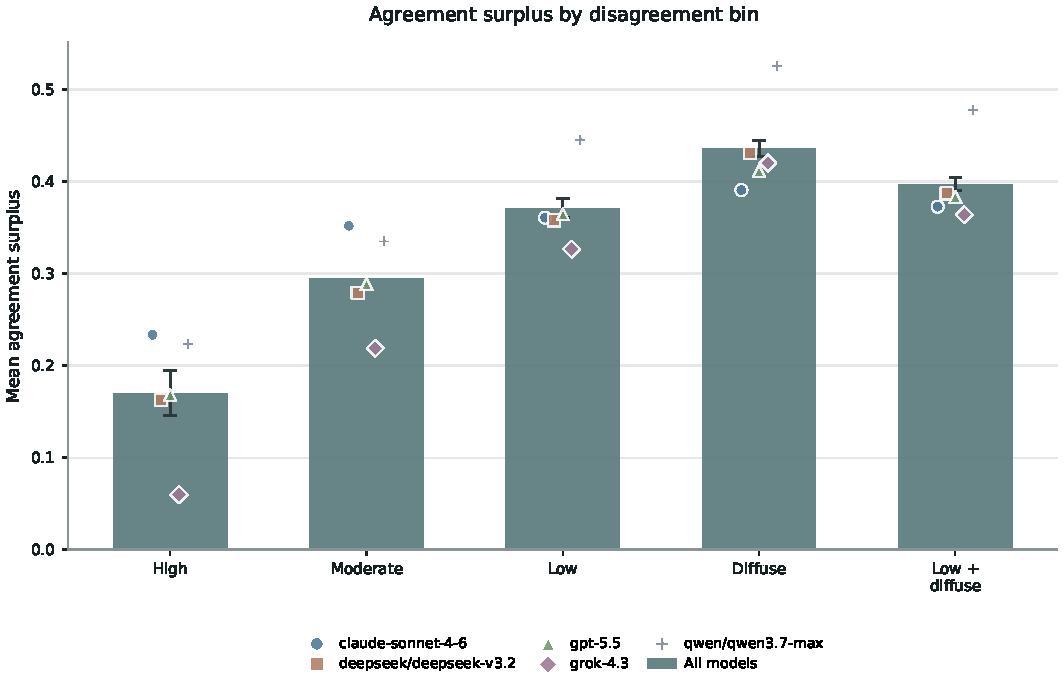
\includegraphics[width=\linewidth,height=0.78\textheight,keepaspectratio]{../figures/final/figure_agreement_surplus_by_bin_model_50k.pdf}
\caption{\textbf{Fig. 2 | Verdict prompts inflate apparent source-community agreement.} Agreement surplus by source-community disagreement bin and model. Bars show aggregate means across the evaluated models; overlaid points show model-level means. Positive values mean that the verdict-mode estimated source-community agreement exceeds source-community support for the model's chosen label. Low-consensus is the primary confirmatory subset; diffuse/no-clear-consensus is secondary evidence; high-consensus is the reference condition. In the low-consensus primary subset, mean agreement surplus was 0.370931 (95\% item-cluster bootstrap CI, 0.361206-0.381114; n = 3,749 item-model rows; Holm-adjusted P = 0.0015 (bootstrap floor)).}
\end{figure}

\begin{figure}[H]
\centering

\includegraphics[width=\linewidth,height=0.78\textheight,keepaspectratio]{../figures/final/figure_distribution_gap_by_bin_model_50k.pdf}
\caption{\textbf{Fig. 3 | Verdict prompts overstate agreement relative to the same model's distribution-mode estimate.} Distribution-agreement gap by source-community disagreement bin and model. Bars show aggregate means across the evaluated models; overlaid points show model-level means. Positive values mean that the verdict-mode agreement estimate exceeds the same model's distribution-mode probability for the same item and verdict-selected label. This endpoint is the cleanest within-model cross-format coherence test because the model, item and selected label are fixed while the elicitation format changes; it does not require perfect calibration of distribution-mode estimates to the SCRUPLES source-community distribution. Low-consensus is the primary confirmatory subset; diffuse/no-clear-consensus is secondary evidence; high-consensus is the reference condition. In the low-consensus primary subset, mean distribution-agreement gap was 0.232687 (95\% item-cluster bootstrap CI, 0.224387-0.241341; n = 3,736 item-model rows; Holm-adjusted P = 0.0015 (bootstrap floor)).}
\end{figure}

\begin{figure}[H]
\centering

\includegraphics[width=\linewidth,height=0.78\textheight,keepaspectratio]{../figures/final/figure_sampling_compression_by_bin_model_50k.pdf}
\caption{\textbf{Fig. 4 | Repeated forced-choice outputs compress source-community disagreement.} Repeated forced-choice concentration by source-community disagreement bin and model. Bars show aggregate means across the evaluated models; overlaid points show model-level means for source-community entropy minus entropy of repeated forced-choice outputs on the five-label scale in bits. Positive values mean that repeated forced-choice outputs are more concentrated than source-community judgments under the study protocol. Low-consensus is the primary confirmatory subset; diffuse/no-clear-consensus is secondary evidence; high-consensus is the reference condition. In the low-consensus primary subset, mean repeated forced-choice concentration was 1.264638 bits (95\% item-cluster bootstrap CI, 1.218425-1.309054; n = 750 item-model summaries; Holm-adjusted P = 0.0015 (bootstrap floor)).}
\end{figure}

\textbf{Table 1 | Model roster and target allocation.} The roster reports the evaluated model IDs, access routes, collection windows and target calls. Provider/route fields record provenance only; provider-family, route and model-family comparisons are outside the analysis. The allocation table reports the frozen study components used for the 50k analysis.

\textbf{a, Model roster and collection windows}

\begin{landscape}
\scriptsize
\setlength{\tabcolsep}{2pt}
\renewcommand{\arraystretch}{1.18}
\begin{longtable}{>{\raggedright\arraybackslash}p{0.15\linewidth}>{\raggedright\arraybackslash}p{0.13\linewidth}>{\raggedright\arraybackslash}p{0.24\linewidth}>{\raggedright\arraybackslash}p{0.18\linewidth}>{\raggedright\arraybackslash}p{0.18\linewidth}>{\raggedright\arraybackslash}p{0.08\linewidth}}
 \toprule
Model ID & Provider/route & API route & First call UTC & Last call UTC & Target calls \\
 \midrule
\path{claude-sonnet-4-6} & Anthropic & \url{https://api.anthropic.com/v1/messages} & \texttt{2026-\allowbreak{}06-\allowbreak{}16T22:\allowbreak{}25:\allowbreak{}08.\allowbreak{}996871+00:\allowbreak{}00} & \texttt{2026-\allowbreak{}06-\allowbreak{}21T15:\allowbreak{}33:\allowbreak{}15.\allowbreak{}162406+00:\allowbreak{}00} & 9,500 \\
\path{deepseek/deepseek-v3.2} & OpenRouter-compatible route & \url{https://openrouter.ai/api/v1/chat/completions} & \texttt{2026-\allowbreak{}06-\allowbreak{}16T22:\allowbreak{}25:\allowbreak{}04.\allowbreak{}892615+00:\allowbreak{}00} & \texttt{2026-\allowbreak{}06-\allowbreak{}21T15:\allowbreak{}33:\allowbreak{}02.\allowbreak{}923140+00:\allowbreak{}00} & 9,500 \\
\path{gpt-5.5} & OpenAI & \url{https://api.openai.com/v1/responses} & \texttt{2026-\allowbreak{}06-\allowbreak{}16T22:\allowbreak{}25:\allowbreak{}12.\allowbreak{}406257+00:\allowbreak{}00} & \texttt{2026-\allowbreak{}06-\allowbreak{}21T15:\allowbreak{}33:\allowbreak{}16.\allowbreak{}432159+00:\allowbreak{}00} & 9,500 \\
\path{grok-4.3} & xAI & \url{https://api.x.ai/v1/responses} & \texttt{2026-\allowbreak{}06-\allowbreak{}17T17:\allowbreak{}55:\allowbreak{}15.\allowbreak{}846572+00:\allowbreak{}00} & \texttt{2026-\allowbreak{}06-\allowbreak{}21T15:\allowbreak{}32:\allowbreak{}59.\allowbreak{}334072+00:\allowbreak{}00} & 9,500 \\
\path{qwen/qwen3.7-max} & OpenRouter-compatible route & \url{https://openrouter.ai/api/v1/chat/completions} & \texttt{2026-\allowbreak{}06-\allowbreak{}16T22:\allowbreak{}25:\allowbreak{}15.\allowbreak{}735026+00:\allowbreak{}00} & \texttt{2026-\allowbreak{}06-\allowbreak{}21T15:\allowbreak{}33:\allowbreak{}13.\allowbreak{}991444+00:\allowbreak{}00} & 9,500 \\
 \bottomrule
\end{longtable}
\normalsize
\setlength{\tabcolsep}{6pt}
\renewcommand{\arraystretch}{1}
\end{landscape}

Temperature was 0.0 for all exported model-roster rows; top-p was blank/null. Provider/route fields record access provenance and are not analysed as cross-provider group effects; model snapshot dates are not inferred beyond the recorded first and last call timestamps. Total target calls were 47,500.

\textbf{b, Target allocation by study component}

\begin{landscape}
\scriptsize
\setlength{\tabcolsep}{2pt}
\renewcommand{\arraystretch}{1.18}
\begin{longtable}{>{\raggedright\arraybackslash}p{0.28\linewidth}>{\raggedright\arraybackslash}p{0.13\linewidth}>{\raggedright\arraybackslash}p{0.13\linewidth}>{\raggedright\arraybackslash}p{0.38\linewidth}}
 \toprule
Component & Unique items & Target calls & Manuscript role \\
 \midrule
Core cross-format & 2,000 & 20,000 & H1a and H1b \\
Repeated sampling & 400 & 20,000 & H1c \\
Paraphrase audit & 250 & 2,500 & Aggregate surface-form evidence \\
Normative certainty & 1,000 & 5,000 & Secondary descriptive analysis \\
Total &  & 47,500 & Frozen 50k target-scoped analysis \\
 \bottomrule
\end{longtable}
\normalsize
\setlength{\tabcolsep}{6pt}
\renewcommand{\arraystretch}{1}
\end{landscape}

\textbf{Table 2 | Primary endpoint estimates, contrasts, confidence intervals and adjusted tests.}

\begin{landscape}
\scriptsize
\setlength{\tabcolsep}{2pt}
\renewcommand{\arraystretch}{1.18}
\begin{longtable}{>{\raggedright\arraybackslash}p{0.16\linewidth}>{\raggedright\arraybackslash}p{0.17\linewidth}>{\raggedright\arraybackslash}p{0.08\linewidth}>{\raggedright\arraybackslash}p{0.17\linewidth}>{\raggedright\arraybackslash}p{0.17\linewidth}>{\raggedright\arraybackslash}p{0.15\linewidth}}
 \toprule
Endpoint & Low-consensus primary mean (95\% CI) & Holm-adjusted P & Diffuse secondary mean (95\% CI) & High-consensus reference mean (95\% CI) & Low--high contrast (95\% CI) \\
 \midrule
Agreement surplus & 0.370931 (0.361206-0.381114) & 0.0015 & 0.435619 (0.427337-0.444341) & 0.169409 (0.145651-0.194624) & 0.201523 (0.174835-0.228568) \\
Distribution-agreement gap & 0.232687 (0.224387-0.241341) & 0.0015 & 0.226556 (0.216740-0.237164) & 0.182842 (0.169762-0.196217) & 0.049845 (0.033774-0.065329) \\
Repeated forced-choice concentration, bits & 1.264638 (1.218425-1.309054) & 0.0015 & 1.507379 (1.452200-1.562768) & 0.563708 (0.495005-0.633547) & 0.700930 (0.618287-0.783543) \\
 \bottomrule
\end{longtable}
\normalsize
\setlength{\tabcolsep}{6pt}
\renewcommand{\arraystretch}{1}
\end{landscape}

Estimates use the frozen 50k target-scoped analysis. Low-consensus values are the primary confirmatory estimates; diffuse/no-clear-consensus values are secondary evidence and remain separate from the primary endpoint definition; high-consensus values are positive estimates for the reference condition. Confidence intervals are item-cluster bootstrap intervals with 2,000 bootstrap iterations. P values are one-sided positive-effect bootstrap P values, Holm-adjusted across the three low-consensus primary endpoints; with 2,000 bootstrap iterations, Holm-adjusted P values are reported at the finite bootstrap floor of 0.0015. A dependence-aware robustness check (model fixed effects plus item-cluster bootstrap, 4,000 iterations) preserved sign and similar magnitude for all three low-consensus endpoints.

\section{Extended Data and Supplementary Information}

The Supplementary Information provides reviewer-facing methodological detail, source-data references and release-safe reproducibility information for the Extended Data figures, Extended Data table and Supplementary Tables. The corresponding source-data files are listed in the Supplementary Information rather than repeated in full in the main manuscript.

\begin{figure}[H]
\centering

\includegraphics[width=\linewidth,height=0.78\textheight,keepaspectratio]{../figures/final/figure_distribution_quality_distances_50k.pdf}
\caption{\textbf{Extended Data Fig. 1 | Distribution-quality diagnostics.} Diagnostic distances and entropy summaries by source-community disagreement bin and model show that distribution-mode outputs varied by item and bin and were not merely uniform or fixed base-rate responses. This is a diagnostic support analysis, not a distribution-prediction benchmark.}
\end{figure}

\begin{figure}[H]
\centering

\includegraphics[width=\linewidth,height=0.78\textheight,keepaspectratio]{../figures/final/figure_paraphrase_audit_effects_50k.pdf}
\caption{\textbf{Extended Data Fig. 2 | Aggregate paraphrase-audit effects.} Aggregate paraphrase-audit agreement surplus and distribution-agreement gap estimates preserve the direction of the main effects. The figure should be interpreted with the limited matched-coverage caveat stated in the Results and Supplementary Information.}
\end{figure}

\begin{figure}[H]
\centering

\includegraphics[width=\linewidth,height=0.78\textheight,keepaspectratio]{../figures/final/figure_validity_rate_by_model_50k.pdf}
\caption{\textbf{Extended Data Fig. 3 | Validity by model and prompt mode.} Primary-valid output rates by model and prompt mode show high validity and limited invalid outputs in the frozen 50k target-scoped analysis.}
\end{figure}

\textbf{Extended Data Table 1 | Validity and exclusion summary.} Reports validity by model/mode, invalid status counts, minimum model/mode validity, refusal count, off-schema count, API errors, terminal failures and repair fields.

\textbf{Supplementary Table 1 | Full model roster, API parameters, model-level endpoints and leave-one-model-out summaries.} Provides model provenance, API-parameter reporting and cross-model consistency checks without making provider-family or model-family claims.

\textbf{Supplementary Table 2 | Source-community distribution smoothing robustness.} Reports raw-proportion, Jeffreys-smoothed and Laplace-smoothed source-community distribution sensitivity checks.

\textbf{Supplementary Table 3 | Annotation and \path{info} robustness.} Reports high-annotation-only, \path{info}-majority exclusion and high-\path{info} exclusion checks.

\textbf{Supplementary Table 4 | Paraphrase audit.} Reports paraphrase target calls, valid outputs, aggregate effects, confidence intervals, chosen-label stability and the matched-coverage caveat.

\textbf{Supplementary Table 5 | Distribution quality and baselines.} Reports distribution-quality diagnostics and uniform, global-base-rate and source-majority-oracle baselines.

\textbf{Supplementary Table 6 | Normative certainty.} Reports the secondary moral-certainty construct; moral certainty is not equivalent to estimated source-community agreement.

\textbf{Supplementary Table 7 | Validity and exclusions.} Reports validity and exclusion summaries and cross-references Extended Data Table 1.

\textbf{Supplementary Table 8 | Model-ready secondary rows.} Provides model-ready secondary rows as transparency files; these files do not contain reported mixed-effects model results.

\textbf{Supplementary Notes.} The Supplementary Information provides supporting methodological detail for prompt and schema reproducibility, source-community preprocessing, item allocation, model provenance, parsing and exclusions, endpoint definitions, bootstrap inference, robustness checks, paraphrase limitations, distribution-quality diagnostics, normative-certainty secondary analysis and public/restricted materials boundaries.
\end{document}
